\section{Automates cellulaires}

\begin{definition}
	Un automate cellulaire est défini par :
	\begin{itemize}
		\item Un entier positif $d$ représentant la dimension de l'espace $(\Z^d)$
		\item Un ensemble fini $S$ d'états
		\item Un ""voisinage"", \ie un ensemble $V = (\vec{v_1},  \vec{v_1}, \ldots ,\vec{v_m})$ de vecteurs de $\Z^d$
		      qui représente la position relative des voisins (relative à la position de la cellule). Les voisins de la
		      cellule $\vec r$ sont $\vec r + \vec {v_1},  \ldots , \vec r + \vec {v_m}$.
		\item Une fonction $f : S ^ m \to S$ de transition locale qui définit l'état d'une cellule à l'instant $t + 1$
		      en fonction des états de ses voisins à l'instant $t$.
	\end{itemize}
\end{definition}

Les automates cellulaires sont synchrones, et homogènes, dans le temps et dans l'espace, \ie,
ils appliquent la règle simultanément a toutes les cellules,
la règle locale de transition ne change pas avec le temps et
ils appliquent la meme règle a toutes les cellules.

\begin{definition}
	Une configuration est une fonction $\Z ^ d \to S$ qui décrit l'état courant de chaque cellule.

	Si $C$ est l'ensemble des configurations, alors un automate cellulaire définit une fonction $G: C \to C$ où si $c \in C$, alors
	$G(c) = c'$ est la configuration obtenue de $c$ en appliquant la règle $f$ à toutes les cellules.

	En général, on itère la fonction $G$ et pour une configuration $c$ on s'intéresse à la suite :
	$$ G^0 (c) = c, G^1 (c), G^2 (c), \ldots \text{ où } G^i (c) = G ( G^{i - 1 }(c))$$
\end{definition}

\begin{definition}
	Un point fixe (ou nature morte) est une configuration $c$ \tlq $\forall k, G^k(c) = c$.
\end{definition}

\begin{definition}
	Une configuration $c$ est dite périodique (dans le temps), ou oscillateur, si $\exists k$ \tq $G^k(c) = c$. Le plus petit
	entier $k$ \tq $G^k(c) = c$ est dit la période d'oscillation.
\end{definition}

\begin{definition}
	Une configuration est dite ultimement fixe si $\exists k$ \tq $\forall j, \ G^{k+j}(c) =  G^{k}(c)$.
\end{definition}


\begin{definition}
	Une configuration est dite ultimement périodique si $\exists k, \exists l>0$ \tq $ G^{k+l}(c) =  G^{k}(c)$,
	\ie à partir de la $k$-ème itération on rentre dans un cycle de longueur $l$.
\end{definition}


\begin{exemple}
	\todo{~}
\end{exemple}


\subsection{Unicité des automates cellulaires}


\begin{theorem}
	Si deux automates cellulaires $A \et B$ réalisent la même fonction $G$, alors $A \et B$ ne peuvent différer que par
	leurs "voisinages" et les deux "voisinages" ne peuvent être différents que par la présence (ou pas) de voisins inutiles (\cad
	des voisins dont l'état n'a aucune influence sur la valeur de $f$).
\end{theorem}


\begin{exemple}
	\todo{~}
\end{exemple}

\subsection{Le jeu de la vie}

\begin{exemple}
	Pour $d = 2$, Game of Life de Conway \cite{conwayGOL} est défini par :
	\begin{itemize}
		\item $S = \set {0,1}$. L'état 0 correspond à l'état d'une cellule \quotes {morte} et 1 à celui d'une cellule \quotes{vivante}.
		\item $V = ((0,1), (1,0), (0,-1), (-1,0), (1,1), (1,-1), (-1,1), (-1,-1))$, dit le voisinage de Moore de rayon 1.
		\item Fonction de transition :
		      \begin{itemize}
			      \item une cellule vivante reste vivante \ssi elle a 2 ou 3 voisins vivants;
			      \item une cellule morte devient vivante \ssi elle a 3 voisins vivants.
		      \end{itemize}
	\end{itemize}

	Une implémentation sur navigateur est disponible sur: \url{https://conwaylife.com/}.
\end{exemple}

\begin{definition}
	On appelle automates cellulaires élémentaires les automates cellulaires qui respectent :
	\begin{itemize}
		\item $d = 1$
		\item $S = \set{0,1}$
		\item $V = (-1,0,1)$
	\end{itemize}

	Il y a exactement $2^8 = 256$ automates élémentaires.
\end{definition}

%\begin{notation}
Wolfram a introduit une numérotation \cite{wolfgramClass} pour les automates cellulaires élémentaires où chaque automate
est associé à un entier entre 0 et 255.

Puisque on peut définir l'automate juste en étudiant son comportement sur les contextes constitués
de trois cellules voisines, il 	suffit d'associer une
étiquette à ce comportement pour caractériser tout l'automate cellulaire. Ainsi, on commence par trier
les huit contextes possibles de trois cellules ainsi :

% From : https://tex.stackexchange.com/questions/320195/is-there-an-implemented-way-to-draw-wolframs-elementary-cellular-automata
\[ \LARGE
	\substack{\blacksquare \blacksquare \blacksquare } \enspace
	\substack{\blacksquare \blacksquare \square } \enspace
	\substack{\blacksquare \square \blacksquare } \enspace
	\substack{\blacksquare \square \square } \enspace
	\substack{\square \blacksquare \blacksquare } \enspace
	\substack{\square \blacksquare \square } \enspace
	\substack{\square \square \blacksquare } \enspace
	\substack{\square \square \square }
\]

Si on considère chaque contexte de trois cellules comme un nombre binaire encodé sur 3 bits, ce tri correspond
à un tri décroissant sur la
valeur de ces nombres (de $7$ à $0$). Pour  chacun de ces contextes on peut donc regarder  quel sera l'état
de la cellule du milieu à la génération suivante.

Par exemple, pour l'automate cellulaire qui réalise la
fonction $f(x_{i-1}, x_i, x_{i+1}) = x_{i-1} \; \mathbf{xor} \; x_{i+1}$ (la valeur de la cellule $i$ à l'instant $t+1$ est le ou exclusif des valeurs des cellules $i-1$ et $i+1$ à l'instant $t$) on a:


\[ \LARGE
	\substack{\blacksquare \blacksquare \blacksquare \\ \square } \enspace
	\substack{\blacksquare \blacksquare \square \\ \blacksquare} \enspace
	\substack{\blacksquare \square \blacksquare \\ \square} \enspace
	\substack{\blacksquare \square \square \\ \blacksquare} \enspace
	\substack{\square \blacksquare \blacksquare \\ \blacksquare} \enspace
	\substack{\square \blacksquare \square \\ \square} \enspace
	\substack{\square \square \blacksquare \\ \blacksquare} \enspace
	\substack{\square \square \square \\ \square}
\]

Maintenant, on peut voir ceci comme un nombre binaire sur 8 bits. Ainsi, pour cet automate cellulaire on obtient :
%ou le $i$-ème bit correspond à la
%nouvelle valeur de la cellule à la $i$-ème position



\[ \LARGE
	\substack{\blacksquare \blacksquare \blacksquare \\ \square \\ 0 } \enspace
	\substack{\blacksquare \blacksquare \square \\ \blacksquare \\ 1} \enspace
	\substack{\blacksquare \square \blacksquare \\ \square \\ 0} \enspace
	\substack{\blacksquare \square \square \\ \blacksquare \\ 1} \enspace
	\substack{\square \blacksquare \blacksquare \\ \blacksquare \\ 1} \enspace
	\substack{\square \blacksquare \square \\ \square \\ 0} \enspace
	\substack{\square \square \blacksquare \\ \blacksquare \\ 1} \enspace
	\substack{\square \square \square \\ \square \\ 0}
\]

Ainsi cet automate est numéroté par $01011010_2 = 90_{10}$. C'est l'automate élémentaire noté $W_{90}$.
%\end{notation}

\subsection{Configurations finies et configurations périodiques}

\begin{definition}
	Soit $s \in S$ un état, et $c$ une configuration, on appelle $s$-support de $c$ l'ensemble des cellules qui ont
	un état différent de $s$.
\end{definition}

\begin{notation}
	Souvent, on impose qu'un état $q_0$ soit un état ""quiescent"" (généralement, c'est l'état 0). Un état quiescent est aussi stable par
	$f$, \ie $f(\underbrace{q_0,\ldots, q_0}_m) = q_0$.
\end{notation}

\begin{definition}
	Si $q_0$ est un état quiescent on appelle configurations finies (ou plus précisément $q_0$-finies) les configurations ayant un $q_0$-support fini.
\end{definition}

Puisque un état quiescent est par stable par définition, il en suit que si $c$ est une configuration finie alors $G(c)$ l'est aussi. Si donc
$F \subset C$ dénote l'ensemble de toutes les configurations finies, la restriction de $G$ à $F$, notée $G_F$, est une fonction de $F$ à $F$.

\begin{definition}
	Soit $\vec v$ un vecteur de $\Z^d$, la translation $\tau_{\vec v}$ est une fonction d'automate cellulaire où le "voisinage" contient seulement
	le vecteur $-\vec v$ et la fonction de transition locale  $f$ est l'identité,
	autrement dit, la valeur d'une cellule $\vec r$ à l'instant $t+1$ est simplement la valeur de la cellule $\vec r - \vec v$ à l'instant $t$.
\end{definition}

\begin{definition}
	On note $\vec \sigma_i = (0,\ldots,0, 1, 0, \ldots, 0)$  le vecteur unitaire qui a la $i$-ème composante égale à 1 et toutes les autres égales
	à 0. Les translation   $\tau_{\vec \sigma_i}$ (pour $i$ dans $\{1, \ldots, d\}$) sont nommées shifts élémentaires.
\end{definition}

Puisque tout vecteur $\vec v$ est une combination linéaire des vecteurs $\vec \sigma_1, \vec \sigma_2, \ldots, \vec \sigma_d$, il en suit que
toute translation peut être exprimée comme une combinaison linaires de shifts élémentaires.

\begin{definition}
	Si $\vec v$ est un vecteur, on dit qu'une configuration $c$ est $\vec v$-périodique si  $c(\vec n) = c (\vec n + \vec v)$ pour tout $\vec n \in \Z ^d$.
\end{definition}

\begin{exemple}
	\todo{~}
\end{exemple}

\begin{definition}
	Une configuration $c$ est dite spatialement périodique si $\exists \vec v$ \tq $c$ est $\vec v$-périodique.
\end{definition}

\begin{definition}
	Une configuration $c$ est dite totalement périodique si $\forall i \in \enum 1 d\exists k_i\in \Z$ \tq $c$ est $k_i\sigma_i$-périodique.
\end{definition}

\begin{prop}
	Si $G$ est la fonction d'un automate cellulaire et $\tau$ une translation, alors $G \circ \tau = \tau \circ G$.
\end{prop}

%\begin{remarque}
Puisque les fonctions d'automates cellulaires commutent avec les translations, il en découle que si $c$ est totalement périodique, alors $G(c)$
est aussi totalement périodique.

Donc si $P$ représente l'ensemble de toutes les configurations (totalement) périodiques, alors la restriction de $G$ à $P$,  notée $G_P$, est une fonction de $P$ à $P$.
%\end{remarque}

Les configurations finies ainsi que les configurations (totalement) périodiques sont importantes parce que elles sont les seules sur
lesquelles on peut tester le comportement d'un automate cellulaire. De plus, comme on le verra dans la suite,  les deux fonctions $G_F$
et $G_P$ donnent des renseignements sur la surjectivité et l'injectivité de $G$.



\subsection{Une topologie sur l'espace des configurations $S^{\Z^d}$}


\begin{definition}
	Soit $c_1,c_2, \ldots$ une suite de configurations, on dit que la suite converge vers
	la configuration $c$ (ou qu'elle a comme limite la configuration $c$) si
	$$ \forall \vec n \in \Z^d, \exists i \mbox{ tel que: } c_j(\vec n) = c(\vec n) \forall j > i$$
\end{definition}

\begin{prop}\label{prop:compact}(Compacité de $S^{\Z^d}.$)

	Toute suite de configurations possède une sous-suite convergente.
\end{prop}

\begin{proof}
	La démonstration est similaire à celle de la factorisation de Ramsay.
	(Une configuration $c $ est une fonction de $\Z^d \to S$ avec $S$ fini, la preuve qu'on a vue est pour les fonctions $\N ^ 2 \to M$, avec $M$ fini).
\end{proof}

\begin{prop}\label{prop:continues}(Les fonctions d'automates cellulaires sont continues.)

	Soit $c_1,c_2, \ldots$ une suite de configurations qui converge vers $c$,
	alors $G(c_1),G(c_2), \ldots$ est une suite de configurations qui converge vers $G(c)$.
\end{prop}

\begin{proof}
	La démonstration n'est pas compliquée et elle est laissée en exercice.
\end{proof}

\begin{prop}\label{prop:dense} (Les configurations finies et totalement périodiques sont denses.)

	Pour toute configuration $c \in S^{\Z^d}$, il existe une suite $c_1,c_2, \ldots$ de configurations finies et une suite  $p_1,p_2, \ldots$
	de configurations (totalement) périodiques telles que :
	$$ \lim_{i \to \infty} c_i = c \et \lim_{i \to \infty} p_i = c $$
\end{prop}

\begin{proof}
	Soit $c$ une configuration quelconque. Soit $\vec {r_0}, \vec {r_1},\ldots$ un dénombrement des cellules de $\Z^d$ (\cad une fonction
	qui attribue un numéro ordinal à chaque $d$-uplet de  $\Z^d$, ceci est possible car  $\Z^d$ est dénombrable)  et pour tout $i \in \N$,
	soit $c_i$ la configuration définie par :

	$$ c_i(r_j) = \left\{ \begin{array}{ll}
			c(r_j) & \text{ si } j \leq i \\
			q      & \text{ sinon }
		\end{array}
		\right.$$
	où $q$ est l'état "quiescent".

	Il est évident que $c_i \in F$ pour tout $i \in \N$ et que $\lim_{i \to \infty} c_i = c$.

	Par ailleurs pour obtenir une suite de configurations périodiques qui convergent vers $c$, on peut construire une suite de configurations
	$p_1, p_2, \ldots $ où $p_i$ coïncide avec $c$ dans l'hypercube centré à l'origine et de coté $2i + 1$ et a une
	période $2i + 1$ dans toutes les directions (on répète cet hypercube à l'infini dans toutes les directions).

	Les configurations $p_i$ sont  périodiques  par construction et  évidemment $\lim_{i \to \infty} p_i = c$.
\end{proof}

\subsection{Injectivité et surjectivité des automates cellulaires}

\begin{definition}
	Un automate cellulaire est dit injectif (respectivement surjectif, bijectif)
	%	$\begin{array}{c}
	%			\text{injectif}  \\
	%			\text{surjectif} \\
	%			\text{bijectif}
	%		\end{array}$
	si sa fonction $G$ est injective  (respectivement surjective, bijective)
	%	$\begin{array}{c}
	%			\text{injective}  \\
	%			\text{surjective} \\
	%			\text{bijective}
	%		\end{array}$
	.
\end{definition}


\begin{theorem} \label{thm:troisprops}
	On a les implications suivantes :
	\begin{enumerate}
		\item $G$ injective $\implies G_F, G_P$ injectives \label{thm:big1}
		\item  $G_F$  surjective ou $G_P$  surjective $\implies G$ surjective \label{thm:big2}
		\item  $G_P$ est injective $\implies G_P$ surjective \label{thm:big3}
	\end{enumerate}
\end{theorem}

\begin{proof}

	\begin{enumerate}
		\item Trivial, la restriction d'une fonction injective est toujours injective.
		\item Dans le cas où $G_F$ est surjective :

		      Soit $c$ une configuration quelconque, montrons que $c$ possède une anti-image.
		      On sait par la Proposition \ref{prop:dense} qu'il existe
		      une suite de configurations finies $c_1, c_2, \ldots , c_m$ \tlq $\lim_{i \to \infty} c_i = c$.
		      Puisque chaque $c_i$ est une configuration finie et comme $G_F$ est surjective,
		      $$\forall i\in \N,  \exists e_i \in F \mbox{ telle que } G_F(e_i) = c_i = G(e_i)$$
		      Soit la suite $e_1, e_2, \ldots $, d'après la proposition  \ref{prop:compact},
		      cette suite doit posséder une  sous-suite convergente. Soit $ e_{i_1}, e_{i_2}, \ldots , e_{i_j} \ldots$ une
		      sous-suite convergente et soit  $e$ sa limite.
		      $G$ est continue par la proposition \ref{prop:continues}, donc la limite de la suite
		      $G(e_{i_1}), G(e_{i_2}), \ldots , G(e_{i_j}) \ldots$ est   $G(e)$.

		      Mais par ailleurs,
		      \begin{eqnarray*}
			      \lim_{j \to \infty} (G(e_{i_j})) &=& \lim_{j \to \infty} (c_{i_j}) \\
			      &=& \lim_{i \to \infty} (c_i) \\
			      &=& c
		      \end{eqnarray*}

		      On a donc $G(e) = c$ et $c$ possède donc une anti-image.\\
		      La preuve est analogue dans l'hypothèse que $G_P$ est surjective.
		\item Soit $c$ une configuration totalement périodique. Par définition
		      $\exists k_1, k_2, \ldots, k_d \in \Z$ tels que:
		      \begin{equation}
			      \forall i \in \enum 1 d, \ \text{la configuration }  c \text{ est } {k_i}\sigma_i\text{-périodique,}
			      \text{ c'est à dire, }
			      c(\vec n) = c(\vec n +  k_i \sigma_i)
			      \label{eq:tmhc}
		      \end{equation}

		      Soit $K$ l'ensemble de toutes les configurations qui satisfont (\ref{eq:tmhc}). On a que $K \subset P$ et $K$ est fini,
		      car chaque configuration de $K$ est uniquement identifiée par l'état des cellules dans un
		      hyper-parallélépipède $d$-dimensionnel de cotés $k_1, k_2, \ldots, k_d$
		      (donc $\abs K = {\abs S}^{k_1k_2\ldots k_d}$)

		      Puisque $G$ commute avec les translations, on a que $G(K) \subseteq K$.

		      Considérons la restriction $\restr G K$. Cette fonction est injective car c'est une restriction de $G_P$ à un
		      sous-ensemble de $P$ et $G_P$ est injective par hypothèse.
		      Mais toute fonction injective sur un ensemble fini est aussi surjective,
		      donc chaque élément de $K$ (dont $c$) a un antécédent dans $K$,
		      donc $\exists e \in K \subsetneq P$ telle que  $G(e) = c$, et donc $G_P$ est surjective.
	\end{enumerate}
\end{proof}

\begin{coro} \label{coro:inj-surj}
	Si un automate cellulaire est injectif, alors il est surjectif (et donc bijectif).
\end{coro}

\begin{proof}
	\begin{eqnarray*}
		G \text{ injective } &\implies& G_P \text{ injective} \reason{\ref{thm:big1} } \\
		&\implies& G_P \text{ surjective} \reason{\ref{thm:big3} } \\
		&\implies& G \text{ surjective} \reason{\ref{thm:big2} }
	\end{eqnarray*}
\end{proof}


\begin{definition}
	On dit qu'un automate cellulaire est réversible s'il est bijectif et si $G^{-1}$ est une fonction d'automate cellulaire.
\end{definition}

\begin{remarque}
	Par définition, si un automate cellulaire est réversible alors il est bijectif.
\end{remarque}

\begin{prop}\label{prop:bij-rev}
	Si $A$ est un automate cellulaire bijectif, alors il est réversible.
\end{prop}

\begin{proof}
	La preuve montre que la fonction $G^{-1}$ est aussi une fonction d'automate cellulaire
	(on peut définir la règle locale d'évolution de  $G^{-1}$ en fonction de l'état de cellules appartenant à un voisinage \emph{borné}).
\end{proof}

\begin{coro}
	$G$ injective $\implies \ G_F$ surjective.
\end{coro}


\begin{proof}
	\begin{eqnarray*}
		G \text{ injective} &\implies& G \text{ bijective} \reason{Cor. \ref{coro:inj-surj} }\\
		&\implies& G \text{ réversible} \reason{Prop. \ref{prop:bij-rev} }
	\end{eqnarray*}
	Si $q$ est l'état "quiescent" pour $G$, alors $q$ est aussi l'état "quiescent" de $G^{-1}$.
	(Si toutes les cellules du voisinage sont à $q$, alors $G^{-1}$ met la cellule à l'état $q$.)

	Donc si $c$ est une configuration finie quelconque,  alors la configuration $e = G^{-1}(c)$ (la configuration obtenue en appliquant
	l'automate inverse) est aussi finie, et alors $G(e) = c$ et $c$ a bien une anti-image finie.
\end{proof}

\todo{add graph}
RM: peut-être mettre le graphe à la fin en sorte de récapitulatif. En particulier l'implication due au  théorème du jardin
d'Eden (GF inj ssi  G surj), n'est pas encore démontrée à ce point.


\subsubsection{Surjectivité et équilibre}
\begin{definition}
	Une configuration qui n'a pas d'anti-image est dite un ""Jardin d'Éden"" ("JDE", ou "GOE" pour Garden of Eden) .
\end{definition}

\begin{remarque}
	L'existence de "Jardins d'Éden" est équivalente à la non surjectivité de l'automate cellulaire.
\end{remarque}

\begin{exemple}
	L'automate élémentaire $W_{110}$ n'est pas surjectif.
	\todo{~}
\end{exemple}


\begin{definition}
	On appelle motif tout ensemble fini $D$ de cellules ainsi que la description des états des cellules de $D$. Formellement, un motif est un
	couple $(D, \varphi)$ où $D$ est un ensemble fini de cellules (dit le domaine du motif) et $\varphi$ une fonction $D \to S$.
\end{definition}


\begin{definition}
	Un motif est dit un \emph{""orphelin""} si toute configuration le contenant est un JDE.
\end{definition}


\begin{exercice}
	Montrer que toute configuration contenant le motif $01010$ est un "Jardin d'Éden" pour $W_{110}$ (le motif 01010 est un orphelin).
\end{exercice}

Dans le cas de $W_{110}$, on a vu que la non-surjectivité et due au fait que la distribution des images des huit contextes n'est pas équilibrée
(il y a cinq contextes ayant comme image $1$ mais seulement trois ayant comme image $0$). Ceci est vrai en général, en effet, d'après la proposition
suivante,  l'équilibre de la distribution est une condition nécessaire (mais pas suffisante) pour la surjectivité,
\begin{prop}
	Si un automate cellulaire est surjectif alors pour tout état $q \in S$ on a : $\abs {f^{-1}(q)}=\abs S ^{n-1}$ où $S$ est l'ensemble de ses états et
	$n$ est la taille du voisinage. En d'autres termes, les images par $f$ des $\abs S ^{n}$ possibles contextes sont distribuées de façon équilibrée sur
	le $\abs S$ états.
\end{prop}

Il existe des automates cellulaires (même élémentaires) qui ont une distribution équilibrées $\abs {f^{-1}(0)}=\abs {f^{-1}(1)}=2^{3-1}= 4$ mais qui ne
sont pas surjectifs, par exemple parce qu'ils n'ont pas une distribution équilibrée pour les quatre  patterns de longueur 2 (00, 01, 10, 11).


\begin{prop}
	Il existe un "JDE" \ssi il existe un "orphelin".
\end{prop}


\begin{proofI}
	\begin{itemize}
		\item \bimpRL\\
		      S'il existe un "orphelin" $D$, alors toute configuration qui inclut l'"orphelin" est un "JDE" par définition.
		\item \bimpLR\\
		      Si un "JDE" existe, alors la fonction $G$ de l'automate n'est pas surjective, et donc par la partie 2 du Théorème  \ref{thm:troisprops}, $G_F$ n'est pas surjective,
		      c'est à dire, $\exists$ une configuration finie qui n'a pas d'anti-image. Le support de cette configuration est  un "orphelin".
	\end{itemize}
\end{proofI}
\begin{definition}
	Deux motifs finis $J_1$ et $J_2$ sont dits jumeaux si ils ont le même domaine et si, en remplaçant $J_1$ par $J_2$ dans
	n'importe quelle configuration qui contient $J_1$, on génère la même configuration.
\end{definition}

\begin{theorem}[du Jardin d'Éden \cite{mooreGOE, myhillGOE}]
	$G_F \text{ injective} \iff G \text{ surjective}$. Autrement dit, un automate cellulaire possède un "JDE" \ssi il possède deux jumeaux.
\end{theorem}



\begin{proofI}
	\begin{itemize}
		\item \bimpLR\\
		      Supposons que $G$ ne soit pas surjective, alors il existe un "JDE" et donc un "orphelin".
		      A partir de l'existence de cet "orphelin", on doit montrer l'existence d'un couple de jumeaux.
		      On ne donnera pas une preuve complète mais on prendra comme exemple l'automate élémentaire $W_{110}$ pour
		      comprendre l'argument de la preuve, qui est un simple argument de comptage.\\
		      On a déjà montré que \emph{01010} est un "orphelin" pour $W_{110}$. Soit $k$ un entier quelconque
		      et considérons  l'ensemble $C_k$ de toutes les configurations finies qui ont un support de taille
		      inférieur ou égale à $5k-2$, alors $\abs {C_k} = 2^{5k-2} = \frac {32^k} 4$

		      Si $c$ est une configuration de $C_k$, alors son image $G(c)$ est une configuration avec un support de taille $5k$.
		      Si on découpe ce support de taille $5k$ en $k$ segments de taille $5$, il y a au plus $31$ choix pour chaque bloc car
		      \emph{01010} est interdit. Alors l'ensemble $G(C_k)$ a une taille d'au plus $31^k$.
		      Or $\frac {32^k} 4 > 31 ^ k$ pour  $k$ suffisamment grand. On a donc que pour $k$ suffisamment grand
		      il y aura plus de configurations
		      dans $C_k$ que dans son image $G(C_k)$, donc il existe des configurations de
		      $C_k$ qui ont la même image (des jumeaux).

		      \todo{RM: Add figure}

		      On pourra s'inspirer de cette exemple pour donner une preuve complète, pour n'importe quel automate qui possède un
		      orphelin dans n'importe
		      quel nombre de dimensions $d > 1$.


		\item \bimpRL\\
		      On donnera la preuve pour le cas $d=2$ car dans ce cas il est possible faire des dessins qui aident à
		      comprendre la demonstration, cependant la généralisation à un nombre quelconque de dimension est immédiate.

		      Soient $J_1$ et $J_2$ deux jumeaux, montrons qu'il existe un orphelin.

		      Soit $n$ un entier tel que:
		      \begin{enumerate}
			      \item le domaine de $J_1$ et $J_2$ est contenu dans un carré de taille $n$;
			      \item le voisinage de chaque cellule ne contient que des cellules à distance inférieure à $n$.
		      \end{enumerate}
		      Soit $m$ un autre entier et considérons l'ensemble $E$ de tous les motifs ayant un domaine inclus
		      dans un carré de taille $mn \times mn$.
		      On veut établir que pour $m$ suffisamment grand au moins l'un de ces motifs n'a pas
		      de prédécesseur (il est donc un orphelin et toute
		      configuration qui le contient est un Jardin d'\'Eden).

		      Le nombre total de ces motifs ayant un domaine inclus
		      dans un carré de taille $mn \times mn$ est évidemment $\abs S  ^{mn \times mn}= {(\abs S  ^{n \times n})}^{m^2}$.

		      Par ailleurs, les prédécesseurs potentielles des motifs de $E$ ont tous un domaine contenu dans
		      un carré de taille $(m+2)n \times (m+2)n$.
		      En effet, si une cellule se trouve en dehors de ce carré, tous ses voisins sont dans l'état quiescent et la cellule
		      restera donc dans l'état quiescent (l'état quiescent est stable).

		      \todo{ADD FIGURE}

		      Soit $P$ l'ensemble des motifs de taille $(m+2)n \times (m+2)n$. Puisque  $J_1$ et $J_2$  ont
		      le même successeur, il suffit de considérer comme prédécesseurs potentiels
		      des motifs de $E$ uniquement les motifs de $P$ qui ne contiennent pas $J_2$.
		      Notons $P'$ l'ensemble de  des motifs de taille $(m+2)n \times (m+2)n$ qui ne contiennent pas $J_2$.

		      L'ensemble $P'$ contient au plus $(\abs S ^{n \times n}-1)^{(m + 2) \times (m + 2)}$ motifs.
		      En effet, ceci est le nombre total de ``pavages'' de la grille de taille $(m+2)n \times (m+2)n$ avec des motifs
		      de taille $n \times n$ différents de $J_2$ et $P'$ est un sous-ensemble des motifs obtenus par ces pavages.

		      Or, pour toute  constante $k > 1$ (et en particulier pour la constante $k=\abs S  ^{n \times n}$) on a :
		      $$\lim\limits_{m \rightarrow +\infty} \frac{k^{m \times m }}{(k-1)^{(m + 2) \times (m + 2)}}= +\infty$$
		      Ceci peut être vérifié facilement en passant  aux exponentielles:
		      $$\lim\limits_{m \rightarrow +\infty} \frac{k^{m \times m }}{(k-1)^{(m + 2) \times (m + 2)}}=
			      \lim\limits_{m \rightarrow +\infty} \frac{(e^{\log k})^{m \times m }}{(e^{\log (k-1)})^{(m + 2) \times (m + 2)}}=
			      \lim\limits_{m \rightarrow +\infty} e^{m^2\log k - (m+2)^2\log (k-1)} $$
		      Il suffit donc d'étudier la limite d'un polynôme de degré 2:
		      $ \lim\limits_{m \rightarrow +\infty} m^2\log k - (m+2)^2\log (k-1)$,  et ce n'est pas difficile de conclure que cette
		      limite est $+\infty$ (le coefficient du terme de degré 2 est positif).

		      %La fonction $f(m) =m^2\log k - (m+2)^2\log (k-1)$ représente une parabole. 
		      %Pour savoir si elle tend vers  $+\infty$ quand $m \rightarrow +\infty$ il suffit d'étudier le signe de sa dérivée 
		      %pour déduire quand elle est croissante.

		      On en déduit qu'au grandir de $m$ la taille de $E$ grandit beaucoup plus vite que la taille de $P'$
		      et donc  que pour un $m$
		      suffisamment grand, il existe des motifs de $E$ qui n'ont pas de prédécesseur dans $P'$, \cad des orphelins.
	\end{itemize}
\end{proofI}



\begin{comment}
Le figures \ref{fig:surj1} et \ref{fig:surj2} résument les relations entre les différentes notions.

\begin{figure}[H]
	\begin{center}
		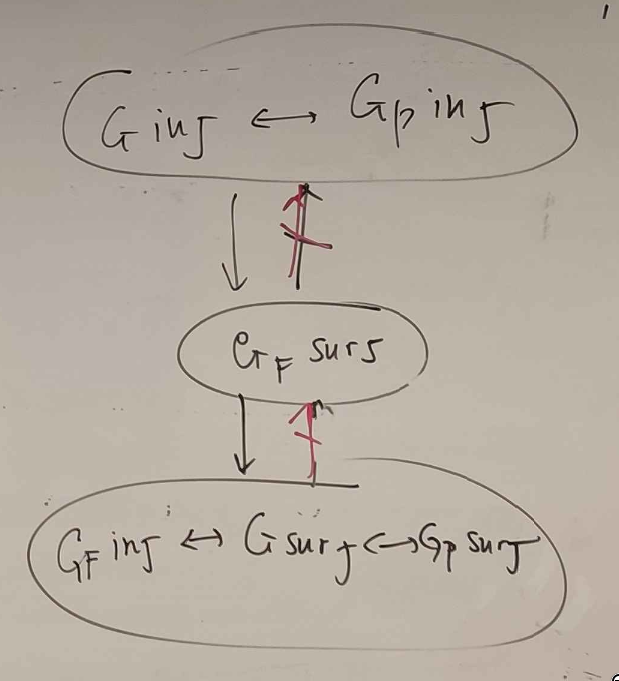
\includegraphics[width=0.3\textwidth]{images/au-cel-d1.png}
	\end{center}
	\caption{Relations avec $d = 1$}\label{fig:surj1}
\end{figure}
\begin{figure}[H]
	\begin{center}
		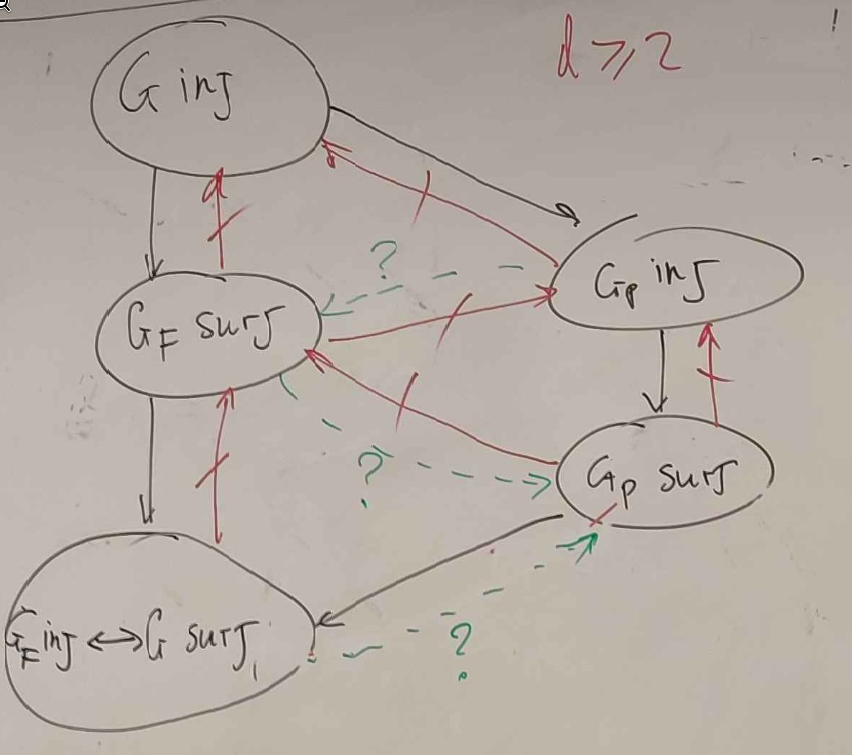
\includegraphics[width=0.3\textwidth]{images/au-cel-d2.png}
	\end{center}
	\caption{Relations avec $d \geq 2$}\label{fig:surj2}
\end{figure}
\end{comment}
